\section{Homework 2}
\subsection{Exercise 2.28}
A matrix is positive semi-definite if we define two matrices symmetric $A$ and $Q$, such that $Q(\textbf{x}) = \textbf{x}^T A \textbf{x} $, $Q$ and $A$ are positive semidefinite if $Q(\textbf{x}) \geq 0$ for all $\textbf{x}$.
\\
In other words, for a matrix $A$ to be positive semidefinite, these two conditions must be satisfied:
\begin{itemize}
  \item $A$ is symmetric
  \item $x^T A x \geq 0$ for all $x$
\end{itemize}
The second condition can be broadened to multiple equivalent definitions:
\begin{itemize}
  \item $x^T A x \geq 0$ for all $x$
  \item All eigenvalues are non-negative
  \item There exists a matrix $B$ s.t. $B^TB = A$
  \item All principal minors are non-negative
\end{itemize}
\subsubsection{n=1}
For $n = 1 $, the cone is defined by the inequality $x_1 \geq 0 $
\subsubsection{n=2}
$x_1x_3 - x_2^2 \geq 0 $ and $x_1,x_3 \geq 0$
\subsubsection{n=3}
All principal minors must be non-negative, so blocking off each row and column of the matrix.
\\ \\
Diagonals: $x_1,x_4,x_6 \geq 0$
\\ \\ 
Full matrix determinant: $x_1 (x_4 x_6 - x_5^2) - x_2 (x_2 x_6 - x_3 x_5) + x_3(x_2 x_5 - x_3 x_4) \geq 0$
2x2 determinants: $x_4 x_6 - x_5^2 \geq 0$, $ x_1 x_6 - x_3^2 \geq 0$ $ x_1 x_4 - x_2^2 \geq 0 $ 
\subsection{Exercise 2.33}
\subsubsection{part a}
A convex cone $K \subseteq \mathbb{R}^n$ is a proper cone if
\begin{itemize}
  \item K is closed (contains its boundary)
  \item K is solid (nonempty interior)
  \item K is pointed (contains no line)
\end{itemize}
For this problem, we must show that the monotone non-negative cone defined as 
\begin{equation}
  K_{m+} = \{ \textbf{x} \in \mathbb{R}^n | x_1 \geq x_2 \geq \dots \geq x_n \geq 0 \}
\end{equation}
is a proper cone.
\\ \\
Proving the first, where $K_{m+}$ is closed and contains its boundary, we first find the boundary of $K_{m+}$. The boundaries are the two vectors in the direction of 
\begin{align}
  \begin{bmatrix}
     1 \\
     0 \\
     \vdots \\
     0
  \end{bmatrix},
  \begin{bmatrix}
    1 \\
    1 \\
    \vdots \\
    1
  \end{bmatrix}
\end{align}
With magnitude $x_1$. These boundaries clearly satisfy the $\geq$ requirements of the set. If one of the conditions was a strict equality, then the convex cone would be open.
\\ \\
Proving the second, since all vectors are contained in between the boundaries, the set is solid.
\\ \\ 
Proving the third, because of the $\geq 0$ requirement, the $\textbf{x}\in \mathbb{R}^n$ of the set also have the $\textbf{x} \succeq 0 $ applicable. Therefore the cone is pointed.
\begin{figure}[htbp]
  \centerline{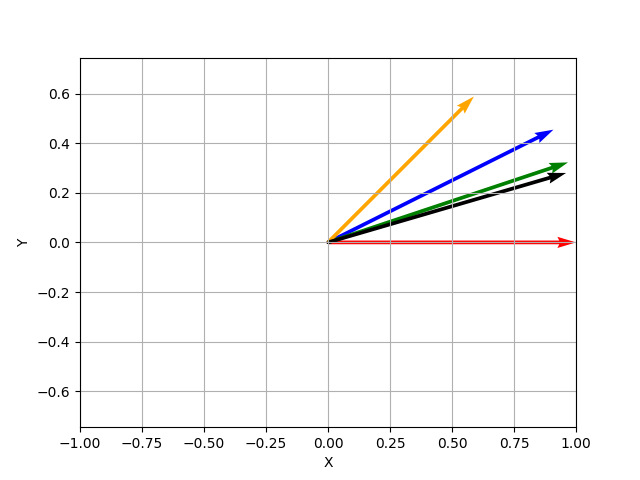
\includegraphics[width=0.50\textwidth]{hw2/images/exercise233cone.png}}
  \caption{Image of a monotone non-negative cone in $\mathbb{R}^2$}
  \label{fig:exercise233cone}
\end{figure}
\subsubsection{part b}
Finding the dual cone $K_{m+}^*$. A dual cone is defined as 
\begin{equation}
  K^* = \{ y | x^T y \geq 0 \text{ for all } x\in K \}
\end{equation}
\begin{gather}
  x^T y \\
  = \sum_{i=1}^n x_i y_i \\
  = (x_1 - x_2)y_1 + (x_2 -x_3)(y_1+y_2) + \dots + (x_{n-1} - x_n)(y_1+\dots + y_n-1) + x_n(y_1+\dots + y_n)
\end{gather}
Since each term of $y$ is getting multiplied by $x_i - x_{i+1}$, and $x_i \geq x_{i+1}$, each $y$ term is getting multiplied by a non-negative $x$ term, so if we want $x^T y \geq 0$ for all x, then we will need in the worst case scenario, for each one of the $y$ terms to be positive.
\begin{equation}
  y_1 \geq 0, y_1 + y_2 \geq 0, y_1 + y_2 + y_3 \geq 0, \dots, \sum_{i=1}^{n} y_i \geq 0
\end{equation}
These conditions are all satisfied when $y_n \geq y_{n-1} \geq \dots \geq y_2 \geq y_1 \geq 0$. Therefore, the dual cone is 
\begin{equation}
  K^* = \{ y \in \mathbb{R}^n | y_n \geq y_{n-1} \geq \dots \geq y_2 \geq y_1 \geq 0\}
\end{equation}
\subsection{Exercise 3.2}
The first function is potentially quasiconvex because the sublevel sets shown are convex. The second function does not seem to have convex sublevel sets. So it is not quasiconvex or quasiconcave.
\subsection{Exercise 3.5}
Showing that the running average of a convex function is also convex. Since $f$ is differentiable, we can attempt to differentiate $F$ twice and evaluate it on the domain of $F$
\begin{equation}
  F(x) = \frac{1}{x} \int_{0}^{x} f(t)dt
\end{equation}

\begin{gather}
  F^\prime(x) = -\frac{1}{x^2} \int_{0}^{x} f(t)dt + \frac{1}{x} \frac{d }{d x}  \int_{0}^{x} f(t)dt \\
= -\frac{1}{x^2} \int_{0}^{x} f(t)dt + \frac{1}{x} (f(x)+ \int_{0}^{x}\frac{d }{d x} f(t)dt) \\
F^\prime(x) = -\frac{1}{x^2} \int_{0}^{x} f(t)dt + \frac{f(x)}{x}
\end{gather}

\begin{gather}
  F^{\prime \prime}(x) = \frac{2}{x^3} \int_{0}^{x} f(t)dt - \frac{1}{x^2} \frac{d }{d x}  \int_{0}^{x} f(t)dt + \frac{f^\prime(x)x - f(x)}{x^2} \\ 
  F^{\prime \prime}(x) = \frac{2}{x^3} \int_{0}^{x} f(t)dt - \frac{f(x)}{x^2} + \frac{f^\prime(x)x - f(x)}{x^2} \\
  F^{\prime \prime}(x) = \frac{2}{x^3} \int_{0}^{x} f(t)dt - \frac{2f(x)}{x^2} + \frac{f^\prime(x)x}{x^2} \\ 
  F^{\prime \prime}(x) = \frac{2}{x^3}( \int_{0}^{x} f(t)dt - f(x)x + \frac{f^\prime(x)x^2}{2}) \\
  = \frac{2}{x^3}( \int_{0}^{x} f(t) - f(x)  - f^\prime(x)(t-x)dt)
\end{gather}
The term $f(t) - f(x) - f^\prime(x)(t-x)$ is always positive because of the definition below for any convex function $f$
\begin{equation}
  f(t) \geq f(x) + f^\prime(x)(t-x)
\end{equation}
Therefore, since the domain of $F$ is confined to all positive numbers, the hessian of $F$ is always greater than zero.
\subsection{Exercise 3.6}
\begin{itemize}
  \item The epigraph of a function is a halfspace if the function is affine. Since the function is linear and infinite, its epigraph is a halfspace. 
  \item If a function is linear then its epigraph is a convex cone.
  \item If a function is piecewise affine, then its epigraph is a polyhedron.
\end{itemize} 

\subsection{Exercise 3.15}
\subsubsection{part a}
Showing that for $x > 0,  u_0(x) = \lim_{\alpha \to 0} u_\alpha (x)$
\begin{equation}
  u_\alpha(x) = \frac{x^\alpha-1}{\alpha}
\end{equation}
L'hopital :)
\begin{equation}
  \lim \frac{x^\alpha-1}{\alpha} = \lim x^\alpha \log x
\end{equation}
This goes to $\log x$ as $\alpha \to 0$
\subsubsection{Part b}
Firstly, $u_\alpha$ is monotonically increasing because the first derivative is
\begin{equation}
  u_\alpha^{\prime} = x^{\alpha-1} 
\end{equation}
Which is always positive. The function is concave since the hessian is 
\begin{equation}
  u_\alpha^{\prime \prime} = (\alpha-1)x^{\alpha-2} 
\end{equation}
Since $0 < \alpha \leq 1$, the function is affine for $\alpha=1$ and concave for all other values of $\alpha$. The equation $u_\alpha(1) = 0 $ is also satisfied since $1^\alpha=1 \forall \alpha$  

\subsection{Exercise 3.16}
Finding whether the functions are convex, concave, quasiconcave, or quasiconvex.

\subsubsection{Part b}
  
\begin{equation}
  f(x_1,x_2)= x_1x_2
\end{equation}
\begin{align}
  \nabla^2 f = 
  \begin{bmatrix}
     0 1 \\
     1 0
  \end{bmatrix}
\end{align}
In reducing to row echelon form, rows 1 and 2 would need to exchange and therefore the matrix is not positive semidefinite and not convex. It is not concave since the negative of the matrix is not positive semidefinite. It is quasiconcave but I didn't really know that.

\subsubsection{Part c}
\begin{equation}
  f(x_1, x_2) = \frac{1}{x_1 x_2}
\end{equation}

\begin{align}
  \nabla^2 f =
  \begin{bmatrix}
     \frac{2}{x_1^3 x_2} \frac{1}{x_1^2 x_2^2} \\
     \frac{1}{x_1^2 x_2^2} \frac{2}{x_1 x_2^3}
  \end{bmatrix}
\end{align}

This function is convex if $\frac{2}{x_1^3 x_2} \geq 0$ and $\frac{3}{x_1^4 x_2^4} \geq 0$. Since $x_1,x_2 \in \mathbb{R}_{++}^2$, the function is convex.

\subsubsection{Part d}
\begin{equation}
  f(x_1, x_2) = \frac{x_1}{x_2}
\end{equation}
\begin{align}
  \nabla^2 f =
  \begin{bmatrix}
     0 \frac{-1}{x^2} \\
     \frac{-1}{x^2} \frac{2x_1}{x_2^3}
  \end{bmatrix}
\end{align}
This function is not convex or concave. I still don't really get quasiconvex or quasiconcave tbh.

\subsubsection{Part e}
\begin{equation}
  f(x_1, x_2) = \frac{x_1^2}{x_2}
\end{equation}
I know this is convex because I watched the lecture but here the hessian
\begin{align}
  \nabla^2 f = 
  \begin{bmatrix}
     \frac{2}{x_2} \frac{-2x_1}{x_2^2} \\
     \frac{-2x_1}{x_2^2} \frac{2x_1^2}{x_2^3}
  \end{bmatrix}
\end{align}
This function is convex when its hessian is positive semidefinite, which is satisfied when $\frac{2}{x_2} \geq 0, \frac{2x_1^2}{x_2^3} \geq 0$ and $\frac{4x_1^2}{x_2^4}   - \frac{4x_1^2}{x_2^4}  \geq 0$. These are always true and therefore $f$ is convex.

\subsection{Exercise 3.18}
Not attempted
\subsection{Exercise 3.24}
Finding if the below probability simplexes are convex, quasiconvex, concave, quasiconcave
\subsubsection{quartile}
\begin{equation}
  \textbf{quartile}(x) = \text{inf} \{ \beta | \textbf{prob}(x\leq \beta ) \geq 0.25\}
\end{equation}
This function is quasiconvex and quasiconcave. It is not convex since it is not continuous
\subsection{Exercise 3.36}
Deriving conjugates of the function
\subsubsection{Max function}
\begin{gather}
  f^*(y) = sup\{y^Tx - f(x)\} \\
  f^*(y) = sup\{y^Tx - max\{x_i\}\} \\
  \frac{d }{d x}  y^Tx - max\{x_i\} = y -
\end{gather}
